
\documentclass[oneside,11pt]{normas-utf-tex} %oneside = para dissertacoes com numero de paginas menor que 100 (apenas frente da folha) 

% force A4 paper format
%\special{papersize=210mm,297mm}

\usepackage{geometry}
\geometry{verbose,a4paper,tmargin=3cm,bmargin=2cm,lmargin=3cm,rmargin=2cm}
%\usepackage[a4paper,top=3cm, bottom=2cm, left=3cm, right=2cm, includeheadfoot, verbose]{geometry}


\usepackage[table]{xcolor}
\usepackage{gensymb}  % Para o (+ ou -), ou \pm

%\usepackage{abntex}
%\usepackage{abntcite}
%\usepackage[scaled]{helvet}
%\renewcommand*\familydefault{\sfdefault} %% Only if the base font of the document is to be sans serif

\usepackage[brazil]{babel} % pacote portugues brasileiro
%\usepackage[T1]{fontenc}
\usepackage[utf8]{inputenc} % pacote para acentuacao direta
\usepackage{amsmath,amsfonts,amssymb} % pacote matematico
\usepackage{graphicx} % pacote grafico
\usepackage[final]{pdfpages} % adicao da ata
\usepackage{hyperref} % gera hiperlinks para o sumario, links, referencias -- deve vir antes do 'abntcite' 
\usepackage{tabularx}
\usepackage{pgfgantt}
\usepackage{rotating}
\usepackage{comment}
\usepackage{subcaption}
\usepackage{mathptmx}
\usepackage{indentfirst} %Indenta o primeiro parágrafo da seção


%\usepackage[scaled]{helvet}
%\renewcommand*\familydefault{\sfdefault} %% Only if the base font of the document is to be sans serif

\renewcommand{\familydefault}{\sfdefault}

\usepackage[alf,abnt-emphasize=bf,bibjustif,recuo=0cm, abnt-etal-cite=2, abnt-etal-list=99]{abntcite} %configuracao correta das referencias bibliograficas.

\usepackage{caption}% http://ctan.org/pkg/caption
%\captionsetup[figure]{justification=raggedleft,singlelinecheck=off}

\usepackage[labelsep=endash]{caption}



% Controle do espaçamento entre um parágrafo e outro:
\setlength{\parskip}{0.1cm}  % tente também \onelineskip

%%%%%% Declarações novas: para mexer no cronograma 

\usepackage{array}
\usepackage{varwidth}

%%%%%%


\DeclareGraphicsExtensions{.pdf,.png,.jpg}

% ---------- Preambulo ----------
\instituicao{Universidade Tecnol\'ogica Federal do Paran\'a} % nome da instituicao
\departamento{Departamento Acadêmico de Informática} % nome do programa
\programa{Curso de Engenharia de Computa\c{c}\~ao} % área ou curso

\documento{Trabalho de Conclusão de Curso}
%\documento{Proposta}
\nivel{Graduação}
\titulacao{Engenheiro de Computação} 

%\titulo{{Controle híbrido de robô seguidor de linha auxiliado por inteligência artificial}} % titulo do trabalho em portugues
%\titulo{{Inteligência artificial aplicada à controle híbrido de robô seguidor de linha (provisorio)}} % titulo do trabalho em portugues
\titulo{{Projeto e Implementação de robô autônomo seguidor de linha}} % titulo do trabalho em portugues

\title{{lalala}} % titulo do trabalho em ingles

\autor{Willian Americano Lopes} % autor do trabalho
\cita{LOPES, Willian Americano} % sobrenome (maiusculas), nome do autor do trabalho

\palavraschave{Quadricóptero. Multi-rotor. VTOL.} % palavras-chave do trabalho
\keywords{Quadrotor. Multi-rotor. VTOL.} % palavras-chave do trabalho em ingles

%\comentario{\UTFPRdocumentodata\ de graduação, apresentado à disciplina de Trabalho de Conclusão de Curso 1, do Curso Superior de Engenharia de Computação do \UTFPRdepartamentodata\ - DAINF - da \ABNTinstituicaodata\ - UTFPR, como requisito parcial para obten\c{c}\~ao do título de ``\UTFPRtitulacaodata\ em Computação''.}
\comentario{Proposta de \UTFPRdocumentodata\ de graduação, apresentada à disciplina de Trabalho de Conclusão de Curso 1, do Curso Superior de Engenharia de Computação do \UTFPRdepartamentodata\ - DAINF - da \ABNTinstituicaodata\ - UTFPR, como requisito parcial para obten\c{c}\~ao do título de ``\UTFPRtitulacaodata\ ''.}


\orientador{Prof. Dr. Fábio Favarim} % nome do orientador do trabalho
\coorientador{Prof. Dr. Eng. César Rafael Claure Torrico} % co-orientador

\local{Pato Branco} % cidade
\data{\the\year} % ano automatico

% desativa hifenizacao mantendo o texto justificado.
% thanks to Emilio C. G. Wille
\tolerance=1
\emergencystretch=\maxdimen
\hyphenpenalty=10000
\hbadness=10000
\sloppy




%---------- Inicio do Documento ----------
\begin{document}


\capa % geracao automatica da capa
\folhaderosto % geracao automatica da folha de rosto

%\termodeaprovacao

%Dedicatória
%\begin{dedicatoria}
%Dedico este trabalho à meus pais, que me proporcionaram este momento (melhorar depois).
%\end{dedicatoria}

%Agradecimentos
%\begin{agradecimentos}
%Incluir os agradecimentos aqui...
%\end{agradecimentos}

%epigrafe
%\begin{epigrafe}
%\textit{``Se enxerguei mais longe, foi porque}\\
%\textit{me apoiei nos ombros de gigantes''}
%\newline \newline \raggedleft Sir Isaac Newton.
%\end{epigrafe}

%resumo
%\begin{resumo}
%Incluir o resumo aqui....
%\end{resumo}

%abstract
%\begin{abstract}
%Include the abstract here
%\end{abstract}

%listas (opcionais, mas recomenda-se a partir de 5 elementos)
%\listadefiguras % geracao automatica da lista de figuras
%\listadetabelas % geracao automatica da lista de tabelas
%\listadequadros % adivinhe :)
%\listadesiglas % geracao automatica da lista de siglas
%\listadesimbolos % geracao automatica da lista de simbolos

% sumario
\sumario % geracao automatica do sumario


%---------- Inicio do Texto ----------
% recomenda-se a escrita de cada capitulo em um arquivo texto separado (exemplo: intro.tex, fund.tex, exper.tex, concl.tex, etc.) e a posterior inclusao dos mesmos no mestre do documento utilizando o comando \input{}, da seguinte forma:


\vspace{-1cm}
\chapter{Introdução} \label{cap:Introducao}

\vspace{-1.5cm} %%%%%%%% Para deixar a introdução no formato padrão
Este capítulo está dividido da seguinte forma: A Seção \ref{Consideracoes_iniciais} apresenta uma visão geral do tema abordado, 
a Seção \ref{Justi} trata da justificativa desta pesquisa, a Seção \ref{limitacoes} trata as limitações do 
projeto e a Seção \ref{objetivos} apresenta os objetivos a serem alcançados neste trabalho. 
% e a seção \ref{organizacao} traz uma visão geral sobre os capítulos posteriores.

%%%%%%%% Utilizar para dar os dois 'enter' antes de seção/ parágrafo
\begin{spacing}{2}\end{spacing} % Está funcionando
\section{Considerações iniciais} \label{Consideracoes_iniciais}    

A robótica é uma das áreas mais promissoras da engenharia, tendo aplicabilidade em várias áreas: de médicas a 
aeroespaciais, buscando oferecer produtividade e flexibilidade à sua aplicação. 
Atualmente é difícil encontrar atividades industriais que não possuam um sistema robótico ou 
automatizado, seja total ou parcial.\par


Devido à ampla aplicabilidade e utilidade que os robôs apresentam foram criadas competições, que visam estimular e 
contribuir com a pesquisa na robótica, tais como:
\begin{itemize}
 \item A \citeonline{robogames} que também é conhecida como ``Olimpíada dos robôs'', em 
que são disputadas mais de cinquenta categorias;
 \item A VEX \citeonline{vex}, a maior competição de robótica do mundo, que contou com 
 1075 times e mais de 15.000 participantes em sua última edição \cite{vex_guiness};
 \item A \citeonline{robocup}, que em 2016 foi sediada em Leipzig, Alemanha;
 \item A \citeonline{robocore}, com eventos realizados no Brasil.\par
\end{itemize}

O WinterChallenge, realizado anualmente pela Robocore, em São Paulo, 
é um dos maiores eventos de robótica da América Latina, contando com a participação de vários países e teve 
mais de mil competidores e cerca de quinhentos robôs na edição de 2016 \cite{maua}.\par

Uma das categorias disputadas é a dos seguidores de linha, na qual os robôs devem seguir, de maneira autônoma, 
um trajeto que é determinado por uma linha. Nessa categoria, se destacam os competidores do Japão, na competição Robogames, 
e do México, na Robocore, estes obtendo os três primeiros lugares na competição WinterChallenge na categoria 
Seguidor de Linha - Pro \cite{winter}. Competindo nesta mesma categoria, 
a equipe Patobots, da Universidade Tecnológica Federal do Paraná 
(\sigla{UTFPR}{Universidade Tecnológica Federal do Paraná}) - 
Câmpus Pato Branco, conquistou o 5º e 6º lugar, com os robôs \textit{Alpha project} e 
\textit{Robbie 3.0}, respectivamente.\par

Com base nesse contexto, este trabalho propõe a construção de um protótipo de um robô seguidor de linha
e o seu respectivo controle, 
visando participar de competições de robótica, como a Robocore.

%% Ficou um pouco forte, eu acho, mas foi solicitação da prof. Kathya para deixar desta forma.
O desenvolvimento deste trabalho contribuirá com a pesquisa que é feita na Universidade Tecnológica Federal do Paraná 
- Câmpus Pato Branco, na área de robótica móvel, em que já foram produzidos 
os trabalhos de \citeonline{allan} e \citeonline{alemao}, os quais servem de base para este trabalho.

\begin{spacing}{2}\end{spacing}
%%%%%%%%%%%%%%%%%%%%%%%%%%%%%%%%%%%%%%%%%%%%%%%%%%%%%%%%%%%%%%%%%%%%%%%%%%%%%%%%%%%%%%%%%%%%%%%%%%%%%%%%%%%%%%%%%%%%%%%%%%
\section{Justificativa} \label{Justi}

O trabalho de \citeonline{allan},
utilizou-se de controle híbrido, o qual 
integrou dinâmicas de controle discreto, como detecção de marcas laterais e a faixa central na pista, e contínuo, 
como o controlador Proporcional Integral Derivativo (\sigla{PID}{Proporcional Integral Derivativo}). Segundo o autor, 
o robô funcionou de acordo com o esperado para um percurso dentro das normas da Robocore, 
tendo alguns problemas relacionados à detecção das marcas laterais quando a pista estava com uma inclinação 
maior que 5º (graus).

O trabalho de \citeonline{alemao} desenvolveu um robô híbrido, realizando um estudo sobre os resultados obtidos por controladores
 PID e \textit{Fuzzy} (lógica difusa), sendo que o controlador PID apresentou melhor desempenho. Segundo o autor, não foi 
obtido sucesso considerável com a técnica \textit{Fuzzy}, que necessitava de um processador com poder computacional maior 
do qual foi utilizado, com memória suficiente para implementar as variáveis de controle.
 Devido às dificuldades encontradas, a comparação dos métodos foi 
realizada no robô 3pi, da Pololu, %\textsuperscript{TM}, %%% comando para o símbolo TM (Trademark)
em que o autor conseguiu uma velocidade de 1 m/s em retas. \par

Comparando os sistemas de controle desenvolvidos verificou-se que o Fuzzy
necessita de um processador bem mais eficiente comparado ao PID, com memória
suficiente para implementar as variáveis de controle, além de maior poder
computacional para processamento matemático, possibilitando o sistema de controle
compensar o erro em tempo hábil.

Com base nos trabalhos de \citeonline{allan} e \citeonline{alemao}, é proposta a modelagem de um novo 
\textit{hardware}, utilizando-se de técnicas de controle híbrido, o qual combina dinâmicas discretas (orientadas a 
eventos) e contínuas (orientadas a tempo) \cite{cassandras}. Também 
propõe-se a utilização de um microcontrolador com Unidade de Ponto-Flutuante 
(\sigla{FPU}{\textit{Floating-Point Unit}}), que pode facilitar a implementação de técnicas mais complexas e 
que exigem maior poder computacional e memória.


\begin{spacing}{2}\end{spacing}
%%%%%%%%%%%%%%%%%%%%%%%%%%%%%%%%%%%%%%%%%%%%%%%%%%%%%%%%%%%%%%%%%%%%%%%%%%%%%%%%%%%%%%%%%%%%%%%%%%%%%%%%%%%%%%%%%%%%%%%%%%
\section{Limitações do Trabalho}\label{limitacoes}

 
Este trabalho apresenta as seguintes limitações:
\begin{enumerate}
 \item Devido à complexidade que é o projeto e a implementação de um robô, este trabalho não se preocupará com 
 o desenvolvimento mecânico do dispositivo, sendo que a estrutura mecânica da mesma será confeccionada 
 sobre uma placa de circuito  impresso;
  \item Devido à dificuldade em encontrar e adquirir peças de alto desempenho, poderão ser utilizadas peças de menor custo, 
  as  quais podem reduzir as capacidades do robô;
 \item O projeto do robô seguidor de linha se aterá ao funcionamento em pistas que seguem as normas da Robocore, podendo 
 apresentar restrições de comportamento e até mesmo não funcionar, caso a pista não esteja no padrão estabelecido. 
\end{enumerate}


\begin{spacing}{2}\end{spacing}
%%%%%%%%%%%%%%%%%%%%%%%%%%%%%%%%%%%%%%%%%%%%%%%%%%%%%%%%%%%%%%%%%%%%%%%%%%%%%%%%%%%%%%%%%%%%%%%%%%%%%%%%%%%%%%%%%%%%%%%%%
\section{Objetivos}\label{objetivos}


\begin{spacing}{2}\end{spacing}
\subsection{Objetivo geral}

Projetar e implementar um protótipo de um robô seguidor de linha, com velocidade máxima próxima a 2 m/s, que seja autônomo,
através da utilização de controle 
híbrido, aperfeiçoando as técnicas desenvolvidas por \citeonline{alemao}.

\begin{spacing}{2}\end{spacing}
\subsection{Objetivos específicos}

\begin{itemize}

 \item Projetar e confeccionar a estrutura do protótipo, visando atender as dimensões especificadas pela Robocore;

  \item Projetar o condicionamento de sinais para os dispositivos a serem utilizados, permitindo 
  uma boa precisão na leitura dos sensores;
 
 \item Implementar o controlador PID, de modo a obter um controlador robusto e estável;
 
 \item Realizar testes com o protótipo em pistas que sigam as normas da Robocore;
 
 \item Implementar um sistema de telemetria, visando obter informações em tempo real do robô;
 
 \item Comparar os resultados obtidos com o de \citeonline{alemao}. 
 
 % A Kathya falou que não é necessário o item de baixo
 %\item Estudar a viabilidade de aplicação de inteligência artificial.
\end{itemize}




\chapter{Referencial Teórico} \label{cap:funda}

\vspace{-2cm} %Deixar no formato certo, 1 'ENTER' após e a seção e 2 'ENTERs' antes da seção

Neste capítulo são apresentados os principais conceitos teóricos relacionados ao desenvolvimento deste trabalho.

\begin{comment}
%%%%%%%%%%%%%%%%%%%%%%%%%%%%%%%%%%%%%%%%%%%%%%%%%%%%%%%%%%%%%%%%%%%%%%%%%%%%%%%%%%%%%%%%%%%%%%%%%%%%%%%%%%%%%%%%%%%%%%%%%%
\vspace{1cm}
\section{Robótica} \label{cap:rob_auto}
% Passar pra frente
A palavra ``Robô'' foi criada pelo escritor tcheco Karel Capek, sendo utilizada em sua peça 
\textit{Rossum's Universal Robots} (\sigla{RUR}{\textit{Rossum's Universal Robots}}), a qual foi 
encenada em 1921, em Praga. Na linguagem eslava, \textit{robota} significa atividade 
forçada ou escrava. Na peça de Capek, os robôs eram pessoas fabricadas artificialmente, ausentes
de emoção \cite{polonskii1996}.\par
A \textit{Robotic Industries Association} (\sigla{RIA}{\textit{Robotic Industries Association}}), 
entidade norte-americana responsável pela indústria de robótica, define um robô industrial como
 \textit{ um manipulador multipropósito reprogramável, controlado automaticamente, programado em três 
 ou mais eixos, os quais podem ser fixos em um lugar ou móveis para aplicações em automação industrial} 
 \cite{RIA_def}.
%\footnote{Fonte em \url{http://www.robotics.org/product-catalog-detail.cfm/productid/2953}. Acesso em: 15 agosto 2016}. 
%Diferentemente do que foi imaginado por Capek, hoje máquinas fazem o trabalho destes seres-humanos.
Diferentemente do que foi imaginado por Capek, são máquinas que realizam o trabalho.

%\begin{comment}
\citeonline{secchi2012} classifica os robôs em três tipos:
\begin{itemize}
 \item Industriais: São formados por estruturas mecâncias articuladas, as quais se movem pelas ordens de um sistema de 
 controle, normalmente um microcontrolador;
 \item Médicos: Também conhecidos como de cooperação ou reabilitação, são os utilizados em cirurgias de alta complexidade e 
 precisão, assim como as próteses inteligentes, que visam manter a aparência e funcionalidade do membro de pessoas com 
 deficiência.;
 \item Móveis: São plataformas mecânicas, que se locomovem através de um certo ambiente e apresentam certa autonomia.
São empregados principalmente em tarefas onde se tem risco à vida humana, como na manutenção de reatores nucleares ou 
exploração de 
minérios, mas também podem ser aplicados na agricultura e no transporte de cargas.
\end{itemize}


\vspace{1cm}
\subsection{Robôs móveis}


%% 	É	AQUI	QUE 	TEM 	QUE	ALTERAR
%% A Kathya falou para colocar outra definição e explicar um pouco melhor.

\end{comment}







%%%%%%%%%%%%%%%%%%%%%%%%%%%%%%%%%%%%%%%%%%%%%%%%%%%%%%%%%%%%%%%%%%%%%%%%%%%%%%%%%%%%%%%%%%%%%%%%%%%%%%%%%%%%%%%%%%%%%%%%%%%
\vspace{1cm}
\section{Regras da Robocore para robôs seguidores de linha} \label{cap:regras_comp}

Na Seção \ref{cap:espc_robocore} e Seção \ref{cap:perc_robocore} são apresentadas as regras relacionadas à 
especificação dos robôs e do percurso, respectivamente, 
para a categoria robô seguidor de linha Pro, em eventos realizados pela \citeonline{RegrasRobocore}.

\vspace{1cm}
\subsection{Especificação dos robôs} \label{cap:espc_robocore}

Para competir na categoria seguidor de linha, os robôs devem ser totalmente autônomos, não podendo ser controlados 
externamente por fio ou por rádio, com exceção para quando este for iniciado. Todos os componentes devem ser embarcados. A 
dimensão máxima permitida é de 250mm   de   comprimento,   250mm   de   largura   e   200mm   de   altura. Não é 
permitido alterar as dimensões do robô durante a partida, assim como alterar o \textit{hardware} ou \textit{software} 
durante a tomada de tempo. Também não é permitida a utilização de mecanismo de sucção, 
que vise aumentar a força normal do robô em relação ao solo.

\vspace{1cm}
\subsection{Especificações do Percurso} \label{cap:perc_robocore}

A pista é feita de uma ou mais placas de \sigla{MDF}{\textit{Medium-Density Fiberboard}} revestidas com uma manta de 
borracha preta, assim, eventualmente serão necessárias emendas para compor a área do percurso. Os robôs, no entanto, 
devem ser capazes de superar os desníveis decorrentes das emendas, que são de aproximadamente 1mm.
Uma linha branca, de 19$\pm$1mm, indica o percurso. Esta linha pode cruzar sobre ela mesma, tendo, neste caso, 
um ângulo de intersecção de 90$\pm$5º (graus), com os 250mm antes e depois do cruzamento sendo retas (conforme pode 
ser visto na Figura \ref{fig:percurso1}). O circuito é totalmente plano, porém podem ocorrer 
inclinações de até 5º.\par



\begin{figure}[h!]
 \centering
 \captionsetup{width=0.37\textwidth,font=footnotesize,textfont=bf}
 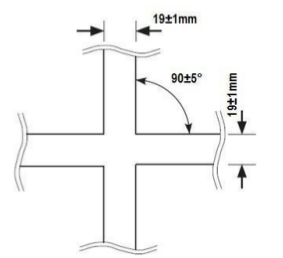
\includegraphics[scale=0.6]{figuras/Percurso1.png}
 \caption{Intersecções no percurso \label{fig:percurso1}}
 \vspace{-0.7cm}
 \caption*{Fonte: Disponível em \cite[p.4]{RegrasRobocore}.}
\end{figure}
%\captionsetup{width=0.50\textwidth, font=footnotesize, textfont=bf}






A área que se estende entre o ponto de partida e o ponto de chegada, considerando 200mm da linha e 200mm a esquerda da linha
 é denominada ``área de partida-chegada'', conforme pode ser visto na Figura \ref{fig:percurso2}.\par

\vspace{0.6cm}
\begin{figure}[h!]
 \centering
 \captionsetup{width=0.55\textwidth,font=footnotesize,textfont=bf}
 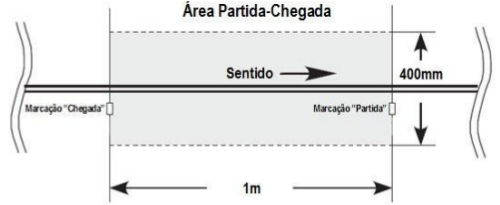
\includegraphics[scale=0.5]{figuras/Percurso2.png}
 \caption{Área de partida-chegada \label{fig:percurso2}}
  \vspace{-0.3cm}
 \caption*{Fonte: Disponível em \cite[p.4]{RegrasRobocore}.}
\end{figure}



%\captionsetup{width=0.50\textwidth, font=footnotesize, textfont=bf}
Quando houver um arco (intersecção entre a faixa branca), o raio deste é de pelo menos 100mm. Quando houver uma 
alteração na curvatura do percurso, deve haver uma marcação no lado esquerdo da linha, como pode ser visto na Figura 
\ref{fig:percurso4}.\par

\begin{figure}[t!]
 \centering
 \captionsetup{width=0.68\textwidth,font=footnotesize,textfont=bf}
 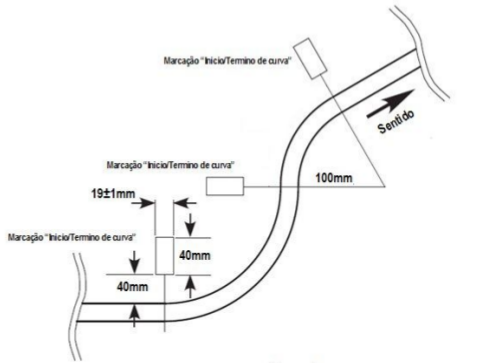
\includegraphics[scale=0.6]{figuras/Percurso4.png}
 \caption{Marcações de sinalização de curvatura \label{fig:percurso4}}
 \vspace{-0.3cm}
 \caption*{Fonte: Disponível em \cite[p.4]{RegrasRobocore}.}
\end{figure}




















%
\chapter{Metodologia} \label{cap:metodologia}
















%\chapter{Recursos de Hardware e Software} \label{cap:materiais}
%\chapter{Materiais} \label{cap:materiais}
\chapter{Materiais} \label{cap:materiais}
\vspace{-2cm}
Neste capítulo serão apresentados os materiais a serem utilizados neste projeto.\newline
%\vspace{1cm}

%%%%%%%%%%%%%%%%%%%%%%%%%%%%%%%%%%%%%%%%%%%%%%%%%%%%%%%%%%%%%%%%%%%%%%%%%%%%%%%%%%%%%%%%%%%%%%%%%%%%%%%%%%%%%%%%%
\section{Microcontrolador} \label{cap:micro}

Será utilizado o \textit{Kit} de desenvolvimento NUCLEO-F303K8, da ST Microelectronics, %\textsuperscript{TM}, 
que possui as seguintes especificações básicas \cite{stm303}:

\begin{itemize}
 \item Microprocessador de arquitetura \textit{Advanced RISC Machine} (\sigla{ARM}{\textit{Advanced RISC Machine}}) Cortex-M4 de 32 bits com FPU;
 \item 72 MHz de frequência máxima de operação;
 \item Instruções de \textit{Digital Signal Processor} (\sigla{DSP}{\textit{Digital Signal Processor}});
 \item 90 DMIPS de desempenho;
 \item 64KB de memória \textit{Flash};
 \item 16KB de SRAM;
 \item 2 módulos \textit{Analog to Digital Converter} (\sigla{ADC}{\textit{Analog to Digital Converter}}) com até 21 canais;
 \item 11 módulos de temporizadores (\textit{timers}).
\end{itemize}%\newline
\vspace{0.5cm}

%%%%%%%%%%%%%%%%%%%%%%%%%%%%%%%%%%%%%%%%%%%%%%%%%%%%%%%%%%%%%%%%%%%%%%%%%%%%%%%%%%%%%%%%%%%%%%%%%%%%%%%%%%%%%%%
\section{Motores CC} \label{cap:motores}
Será utilizado o motor de corrente contínua (\sigla{CC}{Corrente contínua}) 
\textit{High-Power Carbon Brush} (\sigla{HPCB}{\textit{High-Power Carbon Brush}}) modelo 3041 da Pololu, %\textsuperscript{TM} 
\cite{pololu_motor}. Este motor possui alimentação de 12V, caixa de redução 10:1, 3000 
\sigla{RPM}{\textit{Revolutions Per Minute}} e eixo estendido, o qual permite o acoplamento do encoder magnético. 

\vspace{0.5cm}

%%%%%%%%%%%%%%%%%%%%%%%%%%%%%%%%%%%%%%%%%%%%%%%%%%%%%%%%%%%%%%%%%%%%%%%%%%%%%%%%%%%%%%%%%%%%%%%%%%%%%%%%%%%%%%%
\section{Ponte H} \label{cap:ponteh}
Será utilizada uma Ponte H para o controle de velocidade dos motores. O modelo que será utilizado é o TB6612FNG, da 
Toshiba, que é capaz de controlar até dois motores CC com corrente constante de 1,2A \cite{ponte}. 
A velocidade do motor é controlada por \textit{Pulse Width Modulation} (\sigla{PWM}{\textit{Pulse Width Modulation}}).


\vspace{0.5cm}

%%%%%%%%%%%%%%%%%%%%%%%%%%%%%%%%%%%%%%%%%%%%%%%%%%%%%%%%%%%%%%%%%%%%%%%%%%%%%%%%%%%%%%%%%%%%%%%%%%%%%%%%%%%%%%%
\section{Encoder magnético} \label{cap:encoder}
Um \textit{encoder} magnético é um transdutor de movimento, que converte movimentos em informações elétricas, %\cite{}.
sendo possível obter dados como posição e velocidade. Neste trabalho será utilizado o modelo 3081 da 
Pololu, %\textsuperscript{TM}, 
o qual realiza 12 contagens por revolução do eixo e é compatível com o motor 3041 
\cite{pololu_encoder}.

\vspace{0.5cm}

%%%%%%%%%%%%%%%%%%%%%%%%%%%%%%%%%%%%%%%%%%%%%%%%%%%%%%%%%%%%%%%%%%%%%%%%%%%%%%%%%%%%%%%%%%%%%%%%%%%%%%%%%%%%%%%
\section{Sensores de refletância} \label{cap:reflet}
O sensor de refletância é um dispositivo eletrônico que consiste de um \textit{Light Emitter Diode} 
\sigla{LED}{\textit{Light Emitter Diode}} e um fototransistor, medindo assim a refletância de uma superfície. Este circuito 
será utilizado para detectar a linha do percurso. 
O modelo que será utilizado nesse trabalho é o QRE1113P, da Fairchild %\textsuperscript{TM} Semiconductor\cite{reflet}.
Semiconductor\cite{reflet}.
\vspace{0.5cm}

%%%%%%%%%%%%%%%%%%%%%%%%%%%%%%%%%%%%%%%%%%%%%%%%%%%%%%%%%%%%%%%%%%%%%%%%%%%%%%%%%%%%%%%%%%%%%%%%%%%%%%%%%%%%%%%
\section{Placa de circuito impresso} \label{cap:chassi}
O \textit{chassi} do robô, ou seja, a estrutura deste, será confeccionada em uma placa de 
circuito impresso (\sigla{PCB}{\textit{Printed Circuit Board}}) de fenolite.
\vspace{0.5cm}


%%%%%%%%%%%%%%%%%%%%%%%%%%%%%%%%%%%%%%%%%%%%%%%%%%%%%%%%%%%%%%%%%%%%%%%%%%%%%%%%%%%%%%%%%%%%%%%%%%%%%%%%%%%%%%%
\section{Módulo bluetooth} \label{cap:bluetooth}
Será utilizado o módulo \textit{bluetooth} %\textregistered 
HC-05 para a telemetria. Este módulo possuiu a configuração 
mestre-escravo e comunicação \textit{Universal Asynchronous Receiver Transmitter} 
(\sigla{UART}{\textit{Universal Asynchronous Receiver Transmitter}}).

\vspace{0.5cm}


%%%%%%%%%%%%%%%%%%%%%%%%%%%%%%%%%%%%%%%%%%%%%%%%%%%%%%%%%%%%%%%%%%%%%%%%%%%%%%%%%%%%%%%%%%%%%%%%%%%%%%%%%%%%%%%
\section{Rodas} \label{cap:rodas}
Serão utilizadas rodas de poliuretano ou silicone.
\vspace{0.5cm}


%%%%%%%%%%%%%%%%%%%%%%%%%%%%%%%%%%%%%%%%%%%%%%%%%%%%%%%%%%%%%%%%%%%%%%%%%%%%%%%%%%%%%%%%%%%%%%%%%%%%%%%%%%%%%%%
\section{Bateria Lipo} \label{cap:bateria}
Será utilizada uma bateria do tipo Lítio-Polímero (\sigla{Li-Po}{Lítio-Polímero}) de duas céluas, 7,4V, 1300mAh e 
32,5A de corrente máxima de descarga, pois possui alta capacidade de corrente e densidade de carga.
\vspace{0.5cm}

%%%%%%%%%%%%%%%%%%%%%%%%%%%%%%%%%%%%%%%%%%%%%%%%%%%%%%%%%%%%%%%%%%%%%%%%%%%%%%%%%%%%%%%%%%%%%%%%%%%%%%%%%%%%%%%
\section{Conversor Step-Up} \label{cap:stepup}
O conversor \textit{Step-up} que será utilizado é o XL6009, que é um módulo elevador de tensão. Este circuito possui 
eficiência de 94\%, corrente e tensão de saída máxima de 3A e 35V, respectivamente \cite{stepup}.
\vspace{0.5cm}


%\newline


%%%%%%%%%%%%%%%%%%%%%%%%%%%%%%%%%%%%%%%%%%%%%%%%%%%%%%%%%%%%%%%%%%%%%%%%%%%%%%%%%%%%%%%%%%%%%%%%%%%%%%%%%%%%%%%
\section{Esfera deslizante} \label{cap:esfera}
Será utilizada uma esfera deslizante para sustentar a parte frontal do robô e manter os sensores de refletância em sua 
correta posição de funcionamento.
\vspace{0.5cm}


%\newline


%%%%%%%%%%%%%%%%%%%%%%%%%%%%%%%%%%%%%%%%%%%%%%%%%%%%%%%%%%%%%%%%%%%%%%%%%%%%%%%%%%%%%%%%%%%%%%%%%%%%%%%%%%%%%%%
%\section{Step-Down} \label{cap:stepdown}

%\newline




% https://www.pololu.com/product/3038

% https://www.pololu.com/product/3081




\chapter{Cronograma Preliminar} \label{cap:viabi}

%% OBS.: Colocar o \cellcolor dentro de {} para não sobrescrever as linhas da tabela
%%
\vspace{-2cm}
O Quadro \ref{tab:t_cronograma} apresenta um cronograma preliminar do desenvolvimento do Trabalho de Conclusão 
de Curso (\sigla{TCC}{Trabalho de Conclusão de Curso}). 
Na sua elaboração foi considerada a continuação do desenvolvimento
no semestre seguinte, junto à disciplina de TCC 2.

\vspace{1.5cm}
%A Tabela \ref{quad:crono} apresenta um cronograma preliminar do desenvolvimento do \sigla{TCC}{Trabalho de Conclusão de Curso}. Na sua elaboração foi considerado que o autor continuará o desenvolvimento no semestre seguinte, junto com a disciplina de TCC 2.

%\definecolor{cinza}{gray!25}{0.5}
\definecolor{midgray}{gray}{.7}

\begin{quadro}[h]%\footnotesize
% \cline é semelhante ao \hline, porém é possível indicar as colunas que terão essa a linha horizontal
% \multicolumn{10}{c|}{Meses} indica que dez colunas serão mescladas e a palavra Meses estará centralizada dentro delas.
\centering

\resizebox{\columnwidth}{!}{\begin{tabular}[h]{|p{4cm}|c|c|c|c|c|c|c|c|c|c|c|c|}\hline
 & \multicolumn{12}{|c|}{\centering\textbf{Meses}}\\ \cline{2-13}
\raisebox{1.5ex}{\hspace{25pt}\textbf{Atividades}} & 08/16 & 09/16 & 10/16 & 11/16 & 12/16 & 01/17 & 02/17 & 03/17 & 04/17 &
05/17 & 06/17 & 07/17\\ \hline

Elaboração e entrega da proposta & {\cellcolor{midgray}} & {\cellcolor{midgray}} &  &  &  &  &  &  &  &  &  &  \\ \hline
Revisão bibliográfica & {\cellcolor{midgray}} & {\cellcolor{midgray}} & {\cellcolor{midgray}} & {\cellcolor{midgray}} &  &  &  &  &  & &  &  \\ \hline
Condicionamento de sinais dos sensores &  &  & {\cellcolor{midgray}} & {\cellcolor{midgray}} & {\cellcolor{midgray}} & &  &  &  &  &  &  \\ \hline
Projeto do protótipo &  & {\cellcolor{midgray}} & {\cellcolor{midgray}} & {\cellcolor{midgray}} & {\cellcolor{midgray}} & {\cellcolor{midgray}} &  &  &  &  &  &  \\ \hline
Projeto do controlador &  &  & {\cellcolor{midgray}} & {\cellcolor{midgray}} & {\cellcolor{midgray}} & {\cellcolor{midgray}} & &  &  &  &  &  \\ \hline
Desenvolvimento do sistema de telemetria &  &  & {\cellcolor{midgray}} & {\cellcolor{midgray}} & {\cellcolor{midgray}} &  &  &  &  &  &  & \\ \hline
Elaboração e apresentação do TCC 1 &  &  & {\cellcolor{midgray}} & {\cellcolor{midgray}} & {\cellcolor{midgray}} &  &  &  &  &  &  &  \\ \hline
Confecção do protótipo &  &  &  &  &  & {\cellcolor{midgray}} & {\cellcolor{midgray}} & {\cellcolor{midgray}} & &  &  &  \\ \hline
Implementação do controlador &  &  &  &  &  & {\cellcolor{midgray}} & {\cellcolor{midgray}} & {\cellcolor{midgray}} &  &  &  &  \\ \hline
Integração do sistema &  &  &  &  &  &  & {\cellcolor{midgray}} & {\cellcolor{midgray}} & {\cellcolor{midgray}} & {\cellcolor{midgray}} & {\cellcolor{midgray}} & \\ \hline
Testes finais de desempenho &  &  &  &  &  &  &  &  &  & {\cellcolor{midgray}} &{\cellcolor{midgray}}& {\cellcolor{midgray}} \\ \hline
Elaboração e apresentação do TCC 2 &  &  &  &  &  &  &  &  &  & {\cellcolor{midgray}} & {\cellcolor{midgray}} & {\cellcolor{midgray}} \\ \hline

\end{tabular} }
\vfill
\caption{Cronograma das atividades previstas}\label{tab:t_cronograma}
\end{quadro} 
%
\chapter{Conclusões} \label{cap:concl}

Neste documento foi mostrada a viabilidade desse projeto para um trabalho de conclusão de curso. Este seria apenas o primeiro passo de uma série de outros projetos que poderiam aproveitar dos resultados obtidos. Há um grande ramo de aplicações para quadricópteros, como no estudo de algoritmos de controle, para estabilização; inteligência artificial, para detecção e desvio de obstáculos; processamento de imagens; sistemas multi-agentes, no estudo de comportamento coletivo; entre outros. Espera-se que, num futuro próximo, muitas outras surjam com os avanços tecnológicos, permitindo um maior tempo de voo e a realização de mais atividades de modo autônomo.


%---------- Referencias ----------
\clearpage % this is need for add +1 to pageref of bibstart used in 'ficha catalografica'.

%\label{bibstart}
%\bibliographystyle{plain}
%\bibliography{bibliografia} % geracao automatica das referencias a partir do arquivo bibliografia.bib
%\label{bibend}

\bibliographystyle{abnt-alf} % Estilo autor-data

%\bibliography{bibliografia.bib}    % As referencias deste testo estão no arquivo bibliografia.bib
\bibliography{bibliografia}    % As referencias deste testo estão no arquivo bibliografia.bib
%\bibliographystyle{abbrv}
%\bibliography{ref.bib}




% --------- Ordenacao Afabetica da Lista de siglas --------
%\textbf{* Observa\c{c}\~oes:} a ordenacao alfabetica da lista de siglas ainda nao eh realizada de forma automatica, porem
% eh possivel se de realizar isto manualmente. Duas formas:
%
% ** Primeira forma)
%    A ordenacao eh feita com o auxilio do comando 'sort', disponivel em qualquer
% sistema Linux e UNIX, e tambem em sistemas Windows se instalado o coreutils (http://gnuwin32.sourceforge.net/packages/coreutils.htm)
% comandos para compilar e ordenar, supondo que seu arquivo se chame 'dissertacao.tex':
%
%      $ latex dissertacao
%      $ bibtex dissertacao && latex dissertacao
%      $ latex dissertacao
%      $ sort dissertacao.lsg > dissertacao.lsg.tmp
%      $ mv dissertacao.lsg.tmp dissertacao.lsg
%      $ latex dissertacao
%      $ dvipdf dissertacao.dvi
%
%
% ** Segunda forma)
%\textbf{Sugest\~ao:} crie outro arquivo .tex para siglas e utilize o comando \sigla{sigla}{descri\c{c}\~ao}.
%Para incluir este arquivo no final do arquivo, utilize o comando \input{arquivo.tex}.
%Assim, Todas as siglas serao geradas na ultima pagina. Entao, devera excluir a ultima pagina da versao final do arquivo
% PDF do seu documento.


%-------- Citacoes ---------
% - Utilize o comando \citeonline{...} para citacoes com o seguinte formato: Autor et al. (2011).
% Este tipo de formato eh utilizado no comeco do paragrafo. P.ex.: \citeonline{autor2011}

% - Utilize o comando \cite{...} para citacoeses no meio ou final do paragrafo. P.ex.: \cite{autor2011}



%-------- Titulos com nomes cientificos (titulo, capitulos e secoes) ----------
% Regra para escrita de nomes cientificos:
% Os nomes devem ser escritos em italico, 
%a primeira letra do primeiro nome deve ser em maiusculo e o restante em minusculo (inclusive a primeira letra do segundo nome).
% VEJA os exemplos abaixo.
% 
% 1) voce nao quer que a secao fique com uppercase (caixa alta) automaticamente:
%\section[nouppercase]{\MakeUppercase{Estudo dos efeitos da radiacao ultravioleta C e TFD em celulas de} {\textit{Saccharomyces boulardii}}
%
% 2) por padrao os cases (maiusculas/minuscula) sao ajustados automaticamente, voce nao precisa usar makeuppercase e afins.
% \section{Introducao} % a introducao sera posta no texto como INTRODUCAO, automaticamente, como a norma indica.


\end{document}
